\chapter{Media Item Compilation}

% the code below specifies where the figures are stored
\ifpdf
    \graphicspath{{8_media_item_compilation/figures/PNG/}{8_media_item_compilation/figures/PDF/}{8_media_item_compilation/figures/}}
\else
    \graphicspath{{8_media_item_compilation/figures/EPS/}{8_media_item_compilation/figures/}}
\fi

\section{Introduction}

In this chapter, we present and define aesthetic principles
for the automatic generation of media galleries
based on media items retrieved from social networks
that---after a ranking and pruning step---can serve to authentically
summarize events and their atmosphere from a visual
and an audial standpoint.
Mobile devices such as smartphones, together with social networks,
enable people to create, share, and consume media items
like videos or photos.
They accompany their owners almost everywhere
and are thus omnipresent at all sorts of events.
Given a~stable network connection, event-related media items
and microposts are published on social networks
during events and afterwards.
Ranked media items stemming from multiple social networks
can serve to create authentic media galleries
that illustrate events and their atmosphere.
A~key feature for this task is the semantic enrichment
of media items and associated microposts
and the extraction of \textbf{visual}, \textbf{audial},
\textbf{textual}, and \textbf{social} features.
Based on this set of features,
additional \textbf{aesthetic} features
can be defined and exploited to obtain appealing
and harmonic media galleries.

\begin{figure}[htb]
\centering
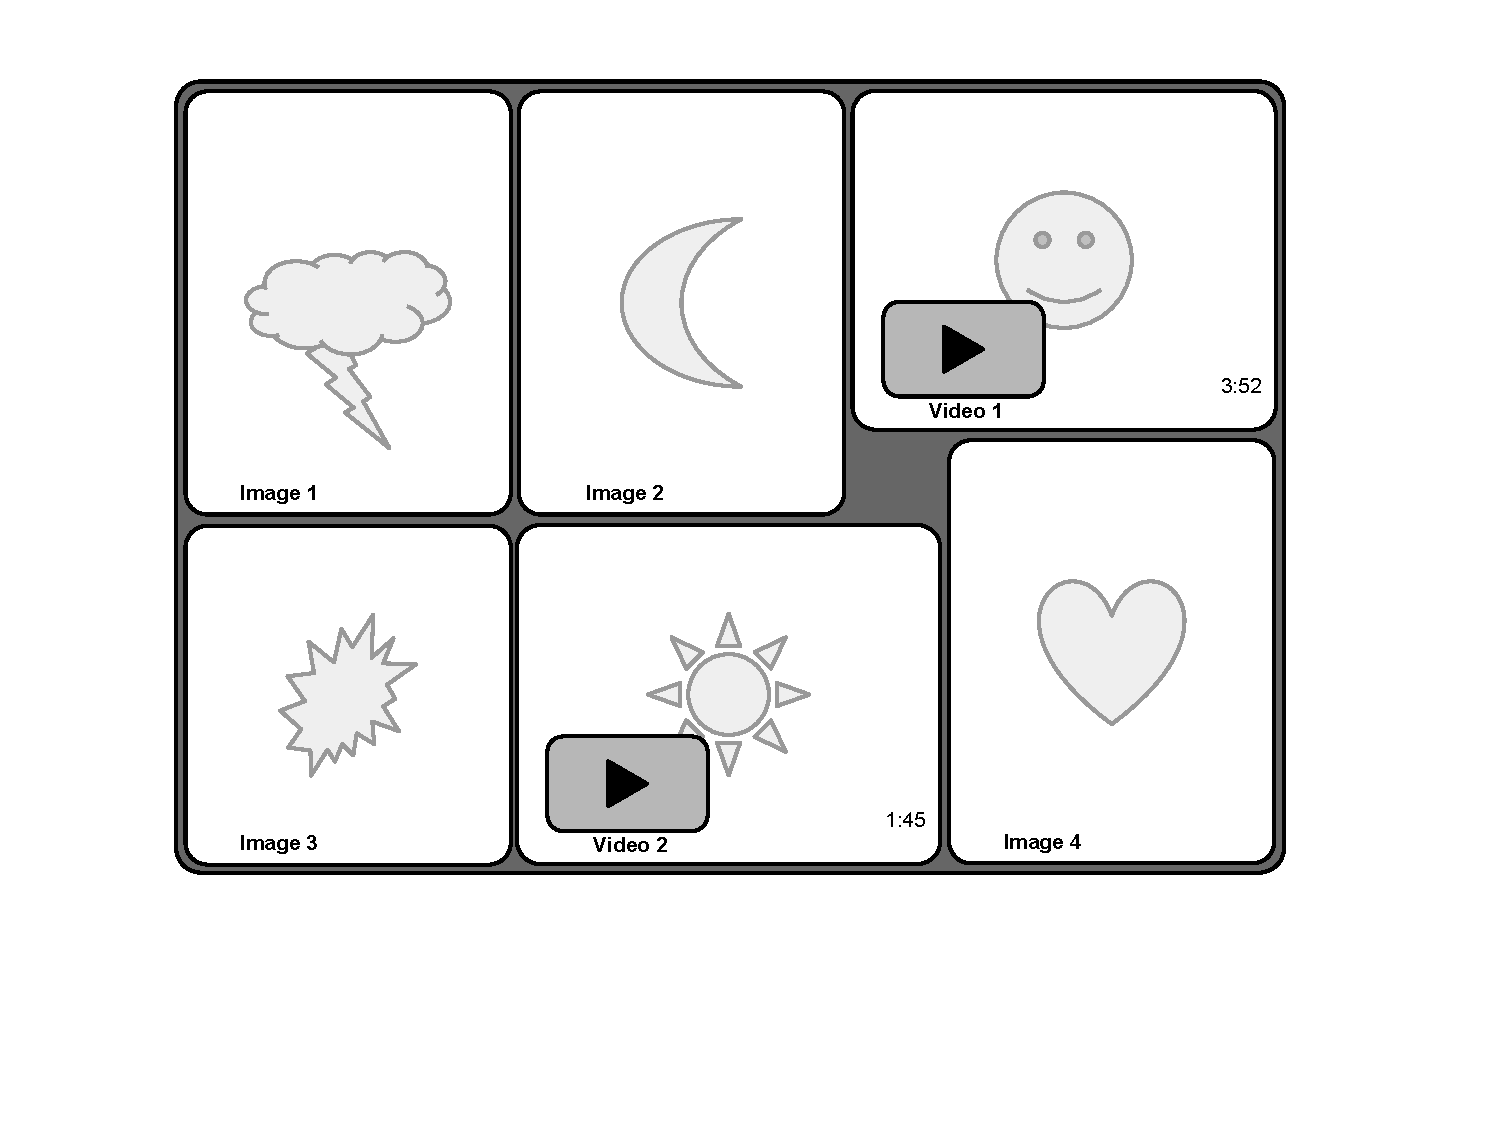
\includegraphics[trim=20mm 40mm 20mm 10mm, clip, width=0.75\columnwidth]{media-gallery.pdf}
\caption{Schematic media gallery with four photos and two videos.}
\label{fig:media-gallery}
\end{figure}

\section{Related Work}
While enormous efforts have been made to extract those features
from media items and microposts on social networks in \emph{isolation},
to the best knowledge of the authors, remarkably less initiatives 
concern the extraction and the application
of all those features \emph{in combination}
for \emph{all} types of media items, including microposts.
In~\cite{Photo2011}, Sandhaus \emph{et al.}\ consider visual and
aesthetic features for the automatic creation of photo books.
Obrador \emph{et al.}\ use visual and aesthetic features
for a category-based approach to automatically assess
the aesthetic appeal of photographs~\cite{Photo2012}.
In~\cite{Playlist2006}, Knees \emph{et al.}\ use audial and textual
features for the automatic generation of music playlists.
Choudhury \emph{et al.}\ show in\cite{Sports2011} how social and textual
features can be used to achieve precise detection results 
of named entities and significant events in sports-related microposts.
In~\cite{YouTube2010}, Davidson \emph{et al.}\ show how visual,
textual, and social features can be used for personalized video recommendations.
A service called Storify~\cite{Storify2011} lets users manually combine
microposts, photos, videos, and other elements onto one page for the purpose
of storytelling or summarizing an event,
and share stories permanently on the Web.
Finally, social networks present photos and videos
often in grid-like galleries\footnote{\url{http://twitpic.com/904yka/full}}, sometimes scaled
based on the amount of comments.
When unique media items have been collected, the remaining task is to summarize events by selecting the most relevant media fragments. Fabro and B\"osz\"orm\'enyi~\cite{Fabro:MMM12} detail the summarization and presentation of events from content retrieved from social media. Nowadays, many domain-specific methods already exhibit good accuracy, for example in the sports domain~\cite{Li1,Li2}. However, the challenge in this field is to find methods that are content-agnostic. Methods that exploit semantic information~(\emph{e.g.}\cite{Chen}) will likely provide high-quality results in the future, but today's most relevant summaries are produced by user interaction~\cite{Olsen}.

\section{Media Gallery Aesthetics}

\noindent \textbf{Definition}
A media gallery in our context is a compilation of photos or videos
retrieved from social networks that are related to a given event.
Given a set $M = \{m_1,..., m_n\}$ of media items related to a certain event,
and given a ranking formula $f$,
the subset $M^\prime \subset M$
is the result after the application of $f$ to $M$: $f(M)=M^\prime$.
Each media item $m_i$ can either be an instance of video or photo.
For each point $t_x$ on a timeline $T$, the state of the media gallery
at $t_x$ is defined for each media item $m_i$
as a set $S_x$ of $n$ tuples $s_{x,i}$, where
$s_{x,i}=\langle \mathit{left}$, $\mathit{top}$, $\mathit{width}$, $\mathit{height}$,
$\mathit{alpha}$, $\mathit{z\mbox{-}index}$, $\mathit{animation}$,
$\mathit{start}$, $\mathit{playing}$, $\mathit{volume} \rangle$.
The first 6~properties are defined as in CSS, the $\mathit{animation}$ property
allows for the definition of CSS transitions
and transformations as defined in~\cite{CSSTransitions2009,CSSTransforms2012},
the $\mathit{start}$ property defines the start time in a video.
A schematic media gallery at $t_x$ can be seen in \autoref{fig:media-gallery}.

\noindent \textbf{Audial aesthetics}
We recall the purpose of our media galleries:
to illustrate an event and its atmosphere.
Audial aesthetics thus consist of aspects like volume level normalization,
avoiding multiple videos playing music in parallel, smooth transitions, \emph{etc}.
We remark that through selective mixing of audio tracks
of event-related videos, ``noise clouds'' very characteristic
for the event atmosphere can be observed.

\noindent \textbf{Visual aesthetics}
Visual aesthetics are determined by the composition, \emph{i.e.},
the relation of photos to videos \emph{globally}, \emph{per coherent scene},
and per \emph{point in time}.
In order not to overcharge the perceptive capacity
of viewers, the number of visible (moving) media items
at a time should be limited.
Depending on the event, a consistent or a contrasty overall
appearance of items may be desired, also for transitions.

\section{Conclusion}
We have introduced media item ranking criteria, and
aesthetic audial and visual principles for media galleries.
In the coming months, we will apply those principles
to a large collection of media items related to events,
and, via multivariate tests, measure user engagement
for different feature configurations.

\section*{Chapter Notes}
This chapter is partly based on the following publications:
\todo{Add publications}